\section{Packet Tracer Design}
For the core of the network of the given bank, we use three main routers each for the HQ and the two branches.
Moreover, we use 17 switches to provide intranet access to each device and provide DHCP availability.

We define two VLANs for the entire network:
\begin{itemize}
  \item \textbf{VLAN 10} for workstations
  \item \textbf{VLAN 50} for servers
\end{itemize}

As per requirement, we restrict all wireless devices connected to an AP to be able to ping only the devices connected to the same AP\@.
Moreover, we restrict that all the other devices in the same or different area cannot ping the wireless devices.

\begin{figure}[H]
  \centering
  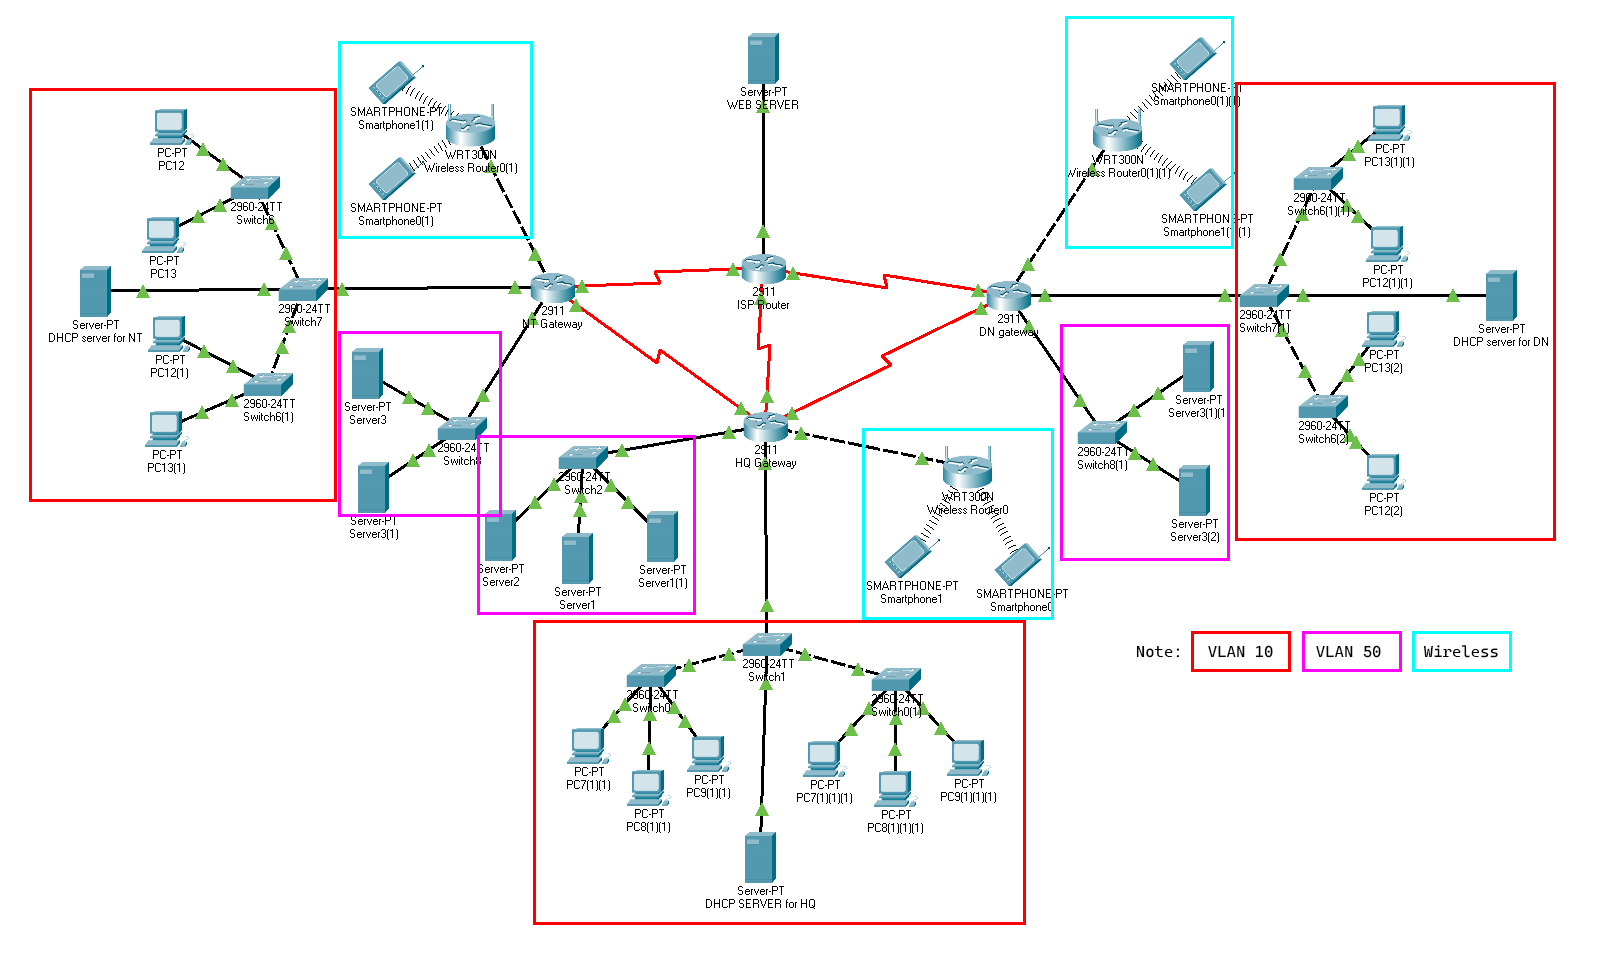
\includegraphics[width=0.8\textwidth]{./assets/pkt1.png}
  \caption{Topological diagram of the whole network}
\end{figure}

\textbf{Note:} This diagram does not contain all the network devices due to the poor runtime optimization of Packet Tracer.
This diagram is scaled down, however the principle and structure of the network should still hold.

\subsection{Switch and VLAN Configuration}
Here, we provide a sample configuration for the HQ.
For the switches in \textbf{VLAN 10}, we configure as follows.

First, we define \textbf{VLAN 10} using the CLI\@.
\begin{code}{Tcl}
  en
  conf t
  vlan 10
  name WorkStationHQ
  int range f0/1-24
  sw mode access
  sw access vlan 10
  int GigabitEthernet0/1
  sw mode access
  sw access vlan 10
  sw mode trunk
  exit
  end
\end{code}

Then, to have the switch provide DHCP service, we use the following commands.
\begin{code}{Tcl}
  en
  conf t
  int range f0/1-24
  sw mode trunk
  int range GigabitEthernet0/1-2
  sw mode access
  sw access vlan 10
  exit
  end
\end{code}

\begin{figure}[H]
  \centering
  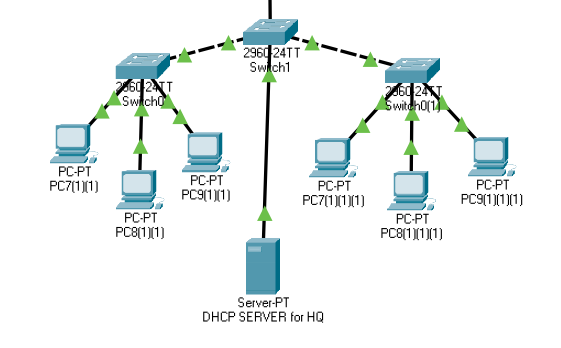
\includegraphics[width=0.8\textwidth]{./assets/pkt2.png}
  \caption{VLAN 10 setup of HQ}
\end{figure}

Now we will configure \textbf{VLAN 50}.
\begin{code}{Tcl}
  en
  conf t
  vlan 50
  name ServerHQ
  int range f0/1-24
  sw mode access
  sw access vlan 50
  int GigabitEthernet0/1
  sw mode access
  sw access vlan 50
  exit
  end
\end{code}

And that is all for the configurations of the network at HQ\@.
The same procedure applies with NT and DN branches.
We only need to change name and interface range.

\subsection{Wireless Router Configuration}
We connect to the default gateway address of the AP to begin configuration.
This address is usually 10.0.1.1, but it can also change if the device has subnet discovery.

\begin{figure}[H]
  \centering
  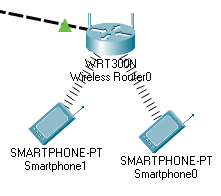
\includegraphics[width=0.4\textwidth]{./assets/ap1.png}
  \caption{Wireless router setup at HQ}
\end{figure}

Then we configure the AP using its GUI\@.
We set the IP address of the AP and the subnet mask as in the picture.
Then we enable the DHCP server, set the start IP address and the maximum number of users.

\begin{figure}[H]
  \centering
  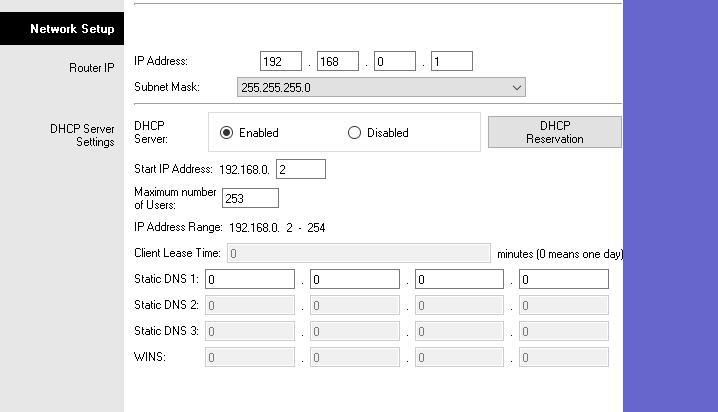
\includegraphics[width=0.8\textwidth]{./assets/wifi1.png}
  \caption{Wireless router setup for HQ}
\end{figure}

And that is the DHCP configuration at the HQ\@.
The same procedure applies with NT and DN branches.

\subsection{OSPF Protocol Setup}
With the use of OSPF protocol, we can manage the connection between the HQ and the branches.

We use the following commands for the gateway routers at HQ, 2 branches and the ISP router.
\begin{code}{Tcl}
  en
  conf t
  router ospf ID
  area AREA
\end{code}
where ID depends on the area.

We assign AREA = 0 as these routers are of the backbone area; ID = 1 for the HQ, 2 for the NT branch, and 3 for the DN branch.

\begin{figure}
    \centering
    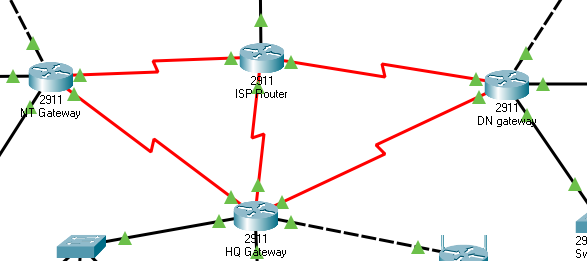
\includegraphics{./assets/core.png}
    \caption{Core network devices}
\end{figure}

\subsection{Security Setup}
In order to restrict the activity at the APs, we use access control list (ACL) to prevent a ping from reaching hosts on other area networks.

We will use the following commands for the 3 gateway routers of the bank.

\begin{code}{Tcl}
  en
  conf t
  ip access-list standard BBBank
  deny 10.0.1.2 0.0.0.0
  deny 10.1.1.2 0.0.0.0
  deny 10.2.1.2 0.0.0.0
  permit 10.0.0.0 0.255.255.255
  deny any
  exit
\end{code}

We continue by applying the ACL to the workstations

\begin{code}{Tcl}
  int GigabitEthernet0/0
  ip access-group BBBank out
  exit
\end{code}

Now we apply the ACL to the servers

\begin{code}{Tcl}
  int GigabitEthernet0/1
  ip access-group BBBank out
  exit
\end{code}

With that done, we can save this config

\begin{code}{Tcl}
  copy running-config startup-config
  write
\end{code}

We will now verify our configuration on ACL\@.

Firstly, we check the router's interface access-list policy

\begin{figure}[H]
  \centering
  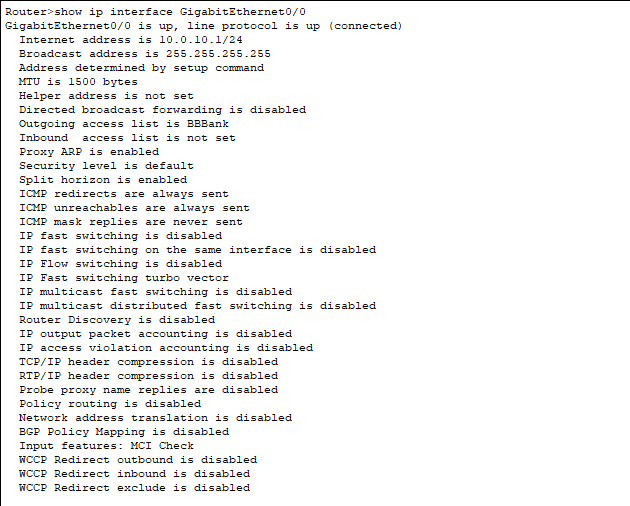
\includegraphics[width=0.8\textwidth]{./assets/acl1.png}
  \caption{ACL policy for the workstations at HQ}
\end{figure}

\begin{figure}[H]
  \centering
  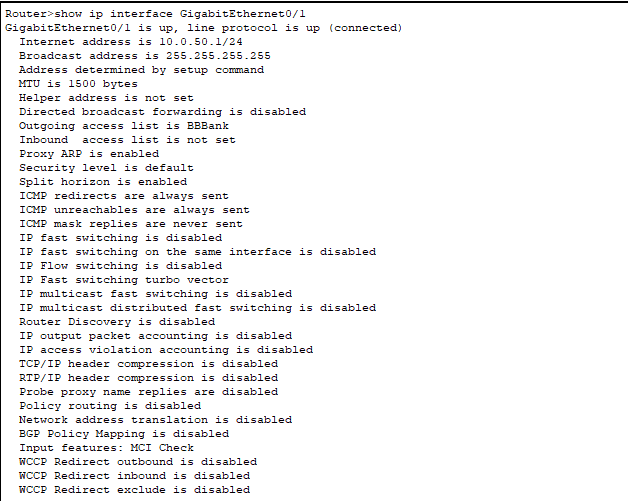
\includegraphics[width=0.8\textwidth]{./assets/acl2.png}
  \caption{ACL policy for the servers at HQ}
\end{figure}

Then we check the ACL group conditions

\begin{figure}[H]
  \centering
  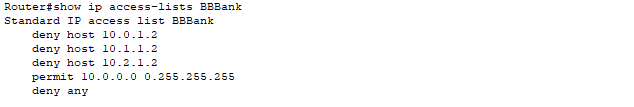
\includegraphics[width=0.8\textwidth]{./assets/acl3.png}
  \caption{IP access list of group BBBank}
\end{figure}
